\documentclass[10pt,pdftex]{report}
\usepackage[T1]{fontenc}
\usepackage[utf8]{inputenc}
\usepackage[magyar]{babel}
\usepackage{graphicx}
\usepackage{amsmath}
\usepackage{amssymb}
\usepackage{multirow}
\usepackage{booktabs}
\usepackage{indentfirst}
\usepackage[a4paper]{geometry}
\usepackage{url}
\usepackage{titling}
\usepackage{float}
\usepackage{xcolor}
    \definecolor{titlebg}{RGB}{128,128,128}

\usepackage{lmodern}
\usepackage{etoolbox}
\patchcmd{\thebibliography}{\chapter*}{\section*}{}{}

\renewcommand{\thesection}{\arabic{section}}


\title{Analóg-digitális átalakító vizsgálata}

%% EZ ALÁBBI KÉT MEZŐT ÉRTELEMSZERŰEN KI KELL TÖLTENI
\author{Bíró Gergő Tamás}
\date{2024. március 11.}


%% FEJLÉC LEÍRÓ, NEM KELL MÓDOSÍTANI
\renewcommand*{\maketitle}{\noindent\colorbox{titlebg}{%
\parbox{\dimexpr\linewidth-2\fboxsep}{\color{white}%
\parbox{\linewidth}{\fontsize{18}{24}\selectfont\sffamily\bfseries\thetitle}%
}}\vskip 1em%
\begin{tabular}{l}%
Mérést végezte: \theauthor \\%
Mérés dátuma: \thedate\\
Jegyzőkönyv végleges változata: \today %
\end{tabular}%
}
%%%%%%%%%%%%%%%%%%%%%

\begin{document}
\maketitle

%% ÉRDEMI MUNKA HELYE
\section*{A mérés célja}
A mérés során a digitális voltmérő működési elvét szeretnénk meghatározni, ezután a rendszer paramétereinek elvi értékét hasonlítjuk össze az adott paraméterre mérésből kapott 
értékekkel, majd a pufferen kijelzett szám értékének a feszültségfüggését vizsgáljuk, és hasonlítjuk össze az elméletben várt értékkel.
\section*{A mérési feladatok dokumentációja, az adatok kiértékelése és az eredmények értelmezése}
\subsection*{A mérés során használt eszközök}
\begin{itemize}
    \item{A digitásis voltmérő áramköre}
    \item{Leibold tápegység}
    \item{Egyenfeszültségű tápegység}
    \item{Oszciloszkóp}
\end{itemize}
\subsection*{A mérés leírása}
A mérés elején a különböző jelek vizsgálatához bemeneti feszültégként $1.21V$-ot tápláltunk be, az oszciloszkópon triggernek beállítottuk az $U_{mono}$ jelet, emellett az oszciloszkóp másik csatornájára sorra végigkapcsoltuk 
a további mérendő jeleket, amelyeknek a tulajdonságait megmértük, és az oszciloszkóp jelét rögzítettük, majd a bementeti jelet kicsit eltérítve $U_{A/D}$ és $U_{mono}$ feszültségek viszonyát vizsgáljuk. Ezután szintén $1.21V$ feszültség mellett az oszciloszkópon az $U_{D/A}$ 
jelre ránagyítva azon a lehető legnagyobb számú lépéshez tartozó feszültségkülönbséget és a lépések számát meghatározzuk. Ezen kívül még az $U_{D/A}$ jelnek több periódusát is megmérjük, 
hogy a periódusidejéből később meghatározzuk az órafrekvenciát. Végül a bemeneti feszültséget $0$-$2.55V$ tartományon változtatva több feszültség mellett vizsgáljuk a pufferen 
megjelenő bináris szám értékét.
\subsection*{A mérés kiértékelése}
\subsubsection*{A rendszerre jellemző adatok}
A mérés során az oszciloszkópon kijelzett adatok néhányszor feltűnően kisebbek voltak az elméleti értéktől, illetve a mérés során a Leibold tápegység feszültségét át kellett 
állítani, mivel az nem a mérés során szükséges feszültségtartományra volt állítva kezdetben. Ezek miatt a következő adatoknak lehetséges, hogy lesz egy szisztematikus hibája.
\newline


A referenciajel amplitúdójára 2.56$V\pm0.02V$ adódott, amely kibahatáron belül van az elméletileg várt 2.55$V$-hoz képest, amely az analóg-digitális átalakító által legnagyobb 
kibocsájtott feszültség nagysága, a jel a periódus elején 0$V$ értéket fesz fel, és közel lineárisan növekszik a periódus végéig, amikor az értéke visszaesik 0$V$-ra. Az oszciloszkópon 
egy periódust mérve a jel szélessége $7.80\pm0.10ms$-nek adódott. Az összehasonlító kimenete egy négyszögjel, melynek amplitúdójára a mért érték $28.4\pm0.2V$, a szélessége szintén 
$7.80\pm0.1ms$, azonban a jel nem ugyanannyi ideig pozitív, és negatív, ezeknek a szakaszoknak a szélességének az arána függ a bemeneti feszültség nagyságától. Az $U_{TTL}$ 
jel alakja, periódusa, és fázisa teljes mértékben megyegyezik az összehasonlító kimeneti jelével, ám az amplitúdója kisebb, értéke $6.24\pm0.08V$. $U_{mono}$ jele szintén 
$7.80\pm0.10ms$ periódosú, feszültségértéke az idő nagy részében 0$V$ körüli értéket vesz fel, ám periódusonként egyszer a feszültsége megnő, és pillanatszerűen felvesz egy nagyobb 
feszültségértéket, amely a mérés során $4.00\pm0.04V$-nak adódott.\newline
\begin{figure}[H]
    \centering
    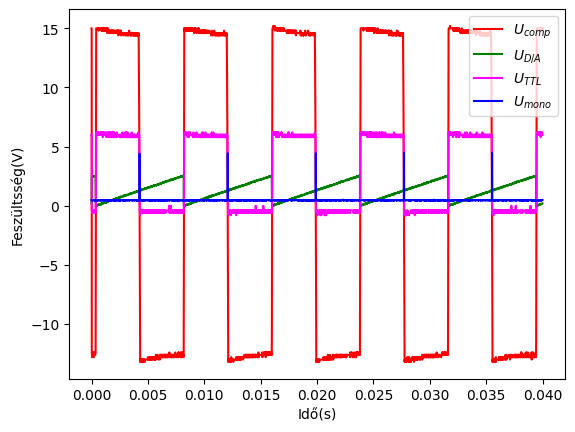
\includegraphics{./Feszultsegek.png}
    \caption{Az egyes jelek feszültségei egyméshoz képest fázishelyesen.}
\end{figure}
A fenti jelalakok segítségével meg lehet állapítani az áramkör működését: \newline
Az órajalet 2 darab 4-bites számlálóból összeállított 8-bites számlálón átvezetve kapott jel segítségével a D/A converter kiad egy kis lépésekből álló jelet, amelynek egy periódusában 
255 lépés van, mivel ez a számláló értékkészlete, annak köszönhetően, hogy az átalakító a feszültsége 0 és 2.55$V$ között lehet, amelynek maximuma az értékkészlet $\frac{1}{100}$-a egy 
lépés során $U_{D/A}$ 0.01$V$-al nő amikor az értékkészlet eléri a maximumát a számláló értéke, és ezzel együtt $U_{D/A}$ értéke is visszaesik 0$V$-ra. A komparátorba ez 
a jel, és a mérendő bemeneti feszültség van petáplálva. Amennyiben a bemeneti jel magasabb a komparátorból ideális esetben az elméletnek megfelelően egy $+15V$-os feszültség 
jön ki. Azonban ha $U_{D/A}$ értéke nagyobb $-15V$-os feszültséget ad ki. $U_{TTL}$ alakja ezzel megegyyezik, és csak az amplitúdója kisebb. $U_{mono}$ feszültségének értéke 
pont abban a pillanatban fog megnőni, amikor $U_{comp}$ előjelet  vált, vagyis amikor $U_{D/A}$ értéke eléri a mérendő bemeneti jel nagyságát, ennek a jelnek a hatására pedig 
a számlálóban az adott pillanatban lévő érték átíródik egy pufferba, a pufferben eltárolt szám pedig a bemeneti feszültség 100-szorosa lesz. \newline


Amennyiben a bemeneti jel nagyságát változtatjuk megfigyelhetjük, hogy $U_{D/A}$ és $U_{mono}$ elcsúsznak egymáshoz képest, ez azért van, mert más bemeneti feszültség esetén más időpontban 
fogja $U_{D/A}$ nagysága meghaladni $U_{be}$ értékét, ha megfigyeljük az ábrákat tényleg megfigyelhetjük, hogy $U_{mono}$ értéke tényleg nagyjából akkor ugrik meg, amikor $U_{D/A}$ 
nagysága eléri a méredő feszültség értékét.
\begin{figure}[H]
    \centering
    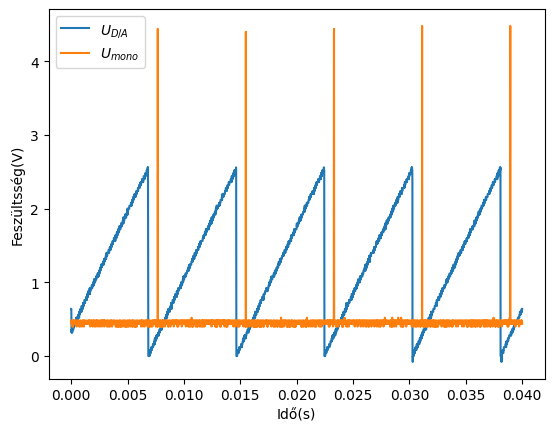
\includegraphics[scale=0.5]{./0_24V.png}
    \caption{$U_{D/A}$ és $U_{mono}$ 0.24$V$-os bemeneti feszültség mellet.}
\end{figure}
\begin{figure}[H]
    \centering
    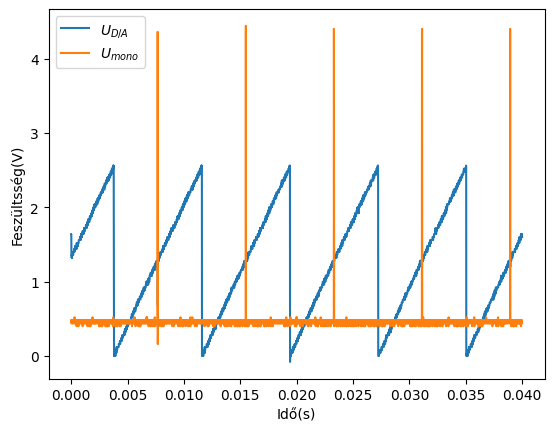
\includegraphics[scale=0.5]{./1_21V.png}
    \caption{$U_{D/A}$ és $U_{mono}$ 1.21$V$-os bemeneti feszültség mellet.}
\end{figure}
\begin{figure}[H]
    \centering
    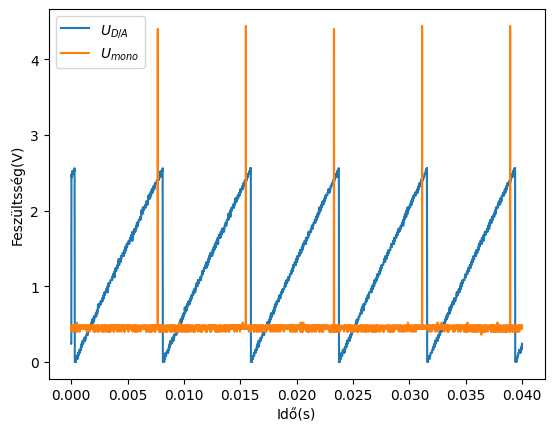
\includegraphics[scale=0.5]{./2_32V.png}
    \caption{$U_{D/A}$ és $U_{mono}$ 2.32$V$-os bemeneti feszültség mellet.}
\end{figure}
\subsubsection*{Rendszerjellemző elméleti értéke}
Az áramkör elemein feltűntetett értékekből $f_{clock}$ azaz az órafrekvencia értéke 32768$Hz$ a számláló értékkészlete $N=2^8-1=255$, és a mérés tartománya $U_{min}=0V$ és $U_{max}=2.55V$ 
közé esik. Ezekből az átalakító két lépése közötti idő $\tau=\frac{1}{f_{clock}}=3.052\cdot 10^{-5}s$, $U_{D/A}$ periódusideje $T=\left(N+1\right)\tau=7.813\cdot 10^{-3}s$, 
a felbontóképessége pedig $k=\frac{U_{max}-U_{min}}{N}=0.01V$
\subsubsection*{Rendszerjellemzők gyakorlati értéke}
$U_{D/A}$ öt periódusát mérve a mért idő $39.2\pm0.2ms$, amiből a periódusideje $T=7.84\pm0.04ms$, amiből pedig $f_{clock}=\frac{256}{T}=32653\pm167Hz$, ahol 
$\Delta f_{clock} = f_{clock}\frac{\Delta T}{T}$. A kvantum meghatározásához az oszciloszkópon $U_{D/A}$ jelére nagyítva a lehető legnagyobb tartományon megmértük a feszültségkülönbséget, 
és az ugrások számát. Végül a mérés során a feszültségkülönbségre $U=316\pm2mV$ adódot, az ehhez tartozó ugrások száma pedig $n=31$ volt, amiből a kavantum mérete 
$k=\frac{U}{n}=0.01019\pm6.45\cdot 10^{-5}V$. Ezeket az előzőekben meghatározott értékekkel összehasonlítva láthatjuk, hogy az előre megadott, és a mért adatok között mindössze 
néhány százalékos különbség van.
\begin{figure}[H]
    \centering
    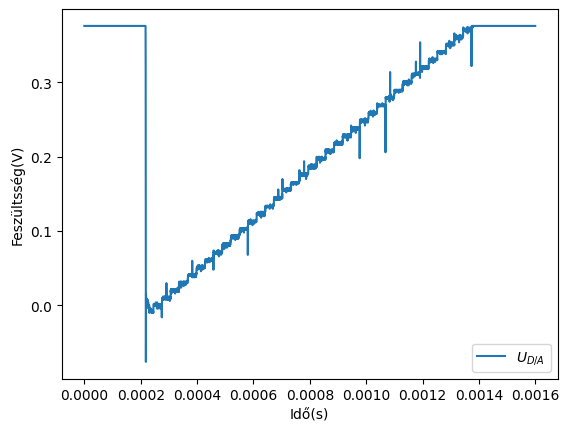
\includegraphics[scale=0.5]{./Nagyitas.png}
    \caption{A kvantum méréséhez használz nagyítás.}
\end{figure}
\subsubsection*{Átvitel}

\section*{Összegzés}

%% IRODALOMJEGYZÉK
%\begin{thebibliography}{9}

%\bibitem{lamport94}
%  Leslie Lamport,
%  \textit{\LaTeX: a document preparation system},
%  Addison Wesley, Massachusetts,
%  2nd edition,
%  1994.
%  \url{https://bla.com}

%\end{thebibliography}

\end{document}
